\section{Bisimulation equivalence}
% no \IEEEPARstart
Bisimulation equivalence (bisimilarity)\footnote{The notion of bisimulation equivalence (bisimilarity) in this chapter 
refers to strong bisimulation equivalence (strong bisimilarity)} is a binary relation between labeled transition systems which associates systems that can simulate each other's behaviour in a stepwise manner. This enables comparison of different transition systems. An alternative perspective is to consider bisimulation equivalence as a relation between states of a single labelled transition system. By considering the quotient transition system under such a relation, smaller models are obtained \cite{ModelChecking}.

The bisimulation equivalence finds its extensive application in many areas of computer science such as concurrency theory, formal verification, set theory, etc. For instance, in formal verification minimization with respect to bisimulation equivalence is used to reduce the size of the state space to be analyzed. Also, bisimulation equivalence is of particular interest in model checking, in specific to check the equivalence of an implementation of a certain system with respect to its specification model.

Our tool implements both options: reducing the size of the state space of a given LTS (minimization modulo bisimilarity) and checking the equivalence of two labeled transition systems modulo bisimilarity.

\subsubsection{Minimization of an LTS modulo bisimilarity.}
The process of reducing the size of the state space of a certain labeled transition system was implemented using an approach which consists of two steps:
\begin{enumerate}
\item Computing strong bisimulation equivalence (strong bisimilarity) for the LTS;
\item Minimizing the LTS to its canonical form using the strong bisimilarity obtained in the first step;
\end{enumerate}

The first step, computing strong bisimulation equivalence, was implemented with two different methods: the so called
naive method and a more efficient method due to Fernandez, both of which can serve as minimization procedures.

The naive algorithm \cite{ReactiveSystems1} for computing bisimulation equivalence stems from the theory underlying 
Tarski's fixed point theorem \cite{ReactiveSystems2}. It has been proven that the strong bisimulation equivalence is 
the largest fixed point of the monotic function $F$ as defined in \cite{ReactiveSystems1} given by Tarsky's fixed 
point theorem. 

The labeled graph was represented as a list of nodes and the following terminology was used:
\begin{itemize}
	\item $S_p=\{(a, q)\}$ - set of pairs $(a, q)$ for state $p$ where $a$ is an outgoing action for $p$ and $q$ is a state
	reachable from $p$ with the action $a$
\end{itemize}

Our Java implementation of the algorithm takes as input an LTS in aldebaran format, generates a corresponding labeled 
graph and then computes the strong bisimulation equivalence as pairs of bisimilar states.

This algorithm has time complexity of $O(mn)$ for a labeled transition system with \emph{m} transitions and \emph{n} 
states. 

The algorithm due to Fernandez exploits the idea of the relationship between strong bisimulation equivalence 
and the relational coarsest partition problem solved by Paige and Tarjan. It represents adaptation of the 
Paige-Tarjan algorithm of complexity $O(m \log n)$ to minimize labeled transition systems modulo bisimulation 
equivalence by computing the coarsest partition problem with respect to the family of binary relations 
$\left(T_a\right)_{a\in A}$ instead of one binary relation, where $T_a=\{(p,q)|(p,a,q)\in T\}$ is a transition 
relation for action $a\in A$ and $T$ is a set of all transitions \cite{PaigeTarjan}\cite{Fernandez}.

The algorithm due to Fernandez in our Java implementation takes an LTS in aldebaran format as an input, generates a 
corresponding labeled graph and then partitions the labeled graph into its coarsest blocks where each block represents 
a set of bisimilar states. Partition is a set of mutually exclusive blocks whose union constitutes the graph universe.

To define graph transitions the following terminology was used: 
\begin{itemize}
	\item $T_a[p]=\{q\}$ - an $a$-transition from state $p$ to state $q$
	\item $T_a{}^{-1}[q]=\{p\}$ - an inverse $a$-transition from state $q$ to state $p$
	\item $T_a{}^{-1}[B]=\cup \left\{T_a{}^{-1}[q],q\in B\right\}$ - inverse transition for block $B$ and action $a$
	\item $W$ - set of sets called splitters that are being used to split the partition
	\item infoB$(a, p)$ - info map for block $B$, state $p$ and action $a$
\end{itemize}

The time complexity of Fernandez's algorithm is $O(m \log n)$ for a labeled transition system 
with $m$ transitions and $n$ states. 

The next step in the reduction of the state space of an LTS uses the bisimulation equivalence computed in the first step in order to minimize the labeled graph. This reduction is implemented as follows:
\begin{enumerate}
	\item If a pair of states $(p, q)$ is bisimilar, then the two states are merged into one single state $k$;
	\item All incoming transitions $r \stackrel{a}{\rightarrow} p$ and $s \stackrel{a}{\rightarrow} q$ are replaced by transitions $r \stackrel{a}{\rightarrow} k$ and $s \stackrel{a}{\rightarrow} k$;
	\item All outgoing transitions $p \stackrel{a}{\rightarrow} r$ and $q \stackrel{a}{\rightarrow} s$ are replaced by transitions $k \stackrel{a}{\rightarrow} r$ and $k \stackrel{a}{\rightarrow} s$;
	\item The duplicate transitions are not taken into consideration.
\end{enumerate}
The procedure is repeated for all pairs of bisimilar states.

The process of reducing a given labeled graph module strong bisimilarity is illustrated below for the labeled graph in Fig. \ref{fig:graph1}.

\begin{figure}[!ht]
\centering
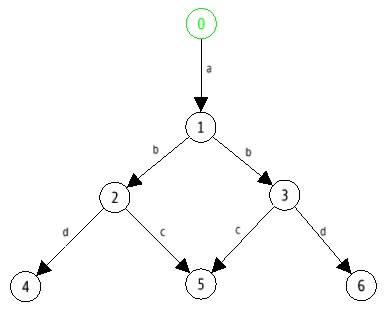
\includegraphics[width=2.3in]{graph1}
\caption{Graph 1}
\label{fig:graph1}
\end{figure}

Applying both the naive and the advanced algorithm due to Fernandez for computing strong bisimulation equivalence for Graph 1, gives the results shown in Table \ref{table1}.
\begin{table}[!ht]
\begin{tabular}{| l | p{10.5cm}| }
  \hline                       
  Algorithm & Graph 1 \\ \hline
  Naive & (2, 3), (3, 2), (4, 5), 
(5, 4), (4, 6), (6, 4), (5, 6), (6, 5), (0, 0), (1, 1), (2, 2), (3, 3), (4, 4), (5, 5), (6, 6) \\ \hline
  Fernandez & \{0\}, \{1\}, \{2\}, \{3\}, \{4, 5, 6\} \\ \hline  
\end{tabular}
\\
\caption{Computing strong bisimularity for Graph 1}
\label{table1}
\end{table}

The results obtained with either of the two algorithms for computing strong bisimilarity are then used as a basis for the reduction of the given graph to its minimal form. Namely, all mutually bisimilar states are merged into a single state and their transitions are updated accordingly. The reduction of Graph 1 to its canonical form with respect to the bisimulation equivalence is given in Fig.  \ref{fig:bisimGraph1}. As it can be seen from the figure, the states 2 and 3 are merged into state 2 in the minimal graph, and states 4, 5 and 6 are merged into state 3 in the minimal graph.

\begin{figure}[!ht]
\centering
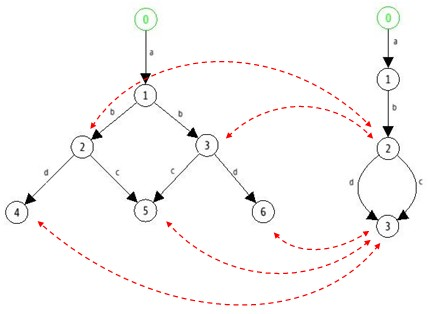
\includegraphics[width=2.8in]{bisimGraph1}.
\caption{Minimized Graph 1}
\label{fig:bisimGraph1}
\end{figure}

\subsubsection{Comparison of two LTSs modulo bisimilarity.}
The idea for the implementation of the equivalence checking of two labeled transition systems modulo strong bisimilarity was based on the following fact: Two labelled transition systems are (strongly) bisimilar iff their initial states are bisimilar \cite{ModellingAndAnalysis}.

That means that in order to check whether two labeled transition systems are bisimilar it is enough to check whether their initial states are bisimilar. This can be done using the following approach:
\begin{enumerate}
	\item The two labeled transition systems are merged into a single transition system
	\item An algorithm for computing the strong bisimilarity is applied to the merged system
	\item A check is performed to see if the initial states belong to the same bisimulation equivalence class
\end{enumerate}

The correctness of the implementation was tested with the use of ltsconvert and ltscompare tools of mCRL2, micro Common Representation Language 2, a specification language that can be used to specify and analyse the behaviour of distributed systems and protocols
\cite{mCRL2Ref}.
